\clearpage

\section{Kroneckerin kokonaisluvut}

Maagikko Kroneckerin mielestä ainoastaan kokonaisluvut ovat normaaleja lukuja. Kaikki muut luvut ovat hänen mielestään paholaisen aikaansaannosta.


Selvitä seuraavista yhtälöistä ne joiden ratkaisut mielyttäisivät Kroneckeriä.

\begin{equation}
2x^2-3=4
\end{equation}
\begin{equation}
x^3-x=0
\end{equation}
\begin{equation}
3a+3=5
\end{equation}
\begin{equation}
x^2-1=0
\end{equation}
\begin{equation}
\cos(x)=-1
\end{equation}
\begin{equation}
\frac{x}{3}=7
\end{equation}
\begin{equation}
-b+4=6
\end{equation}
\begin{equation}
\frac{3x^2-18x+24}{x-4}=0
\end{equation}
\begin{equation}
x^2+1=0
\end{equation}
\begin{equation}
-2x+6x^2=7
\end{equation}
\begin{equation}
\sqrt{x+2}=4
\end{equation}
\begin{equation}
\frac{x^2-4}{x-2}=0
\end{equation}
\begin{equation}
e^{ix}+1=0
\end{equation}

Vihje: Mikäli jokin yhtälöistä ei ratkea helposti, ei kannata huolestua. Joukosta saattaa löytyä kompia...

\begin{figure}[h]
    \centering
    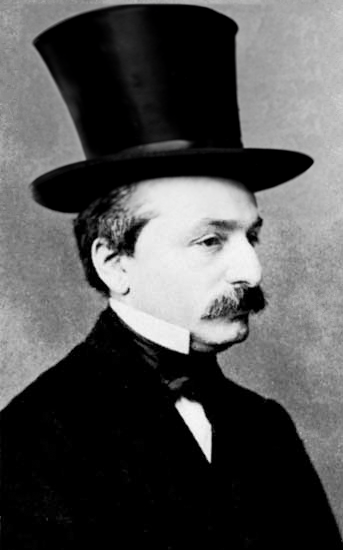
\includegraphics[width=0.15\textwidth]{kuvat/kronecker ja hattu.png}
    \caption*{Leopold Kronecker (1823-1891)}
\end{figure}
